\documentclass[landscape,final,paperwidth=48in,paperheight=33in,fontscale=0.285]{baposter}
%\usepackage{calc,array}
\usepackage{graphicx} % Required for including images
\usepackage{amsmath}  % For typesetting math
\usepackage{amssymb}  % Adds new symbols to be used in math mode
\usepackage{relsize}  % Change size of text /smaller, /larger
\usepackage{multirow} % Allows table cells to span more than one row of the table
\usepackage{rotating} % Rotate figures and tables
\usepackage{bm}       % Allows a math expression to be bold
\usepackage{url}      % Allows email address and websites
\usepackage{gensymb}  % Allows degree symbol
\usepackage{siunitx}  % Scientific notation

\usepackage{float}
\usepackage{caption} % Required for specifying captions to tables and figures
\usepackage{wrapfig} % Wrap text around figure
\usepackage[export]{adjustbox}

%\captionsetup[figure]{font=Large,skip=0pt,labelformat=empty,justification=raggedright,singlelinecheck=false}

\usepackage{multicol} % Required for multiple columns

\usepackage[utf8]{inputenc} %Required for IEEE reference style
\newcommand{\BIBdecl}{\setlength{\itemsep}{-0.25 em}} %Removes line space between references

% Fonts
%\usepackage{times}
%\usepackage{helvet}
%\usepackage{bookman}
\usepackage{palatino}

%\newcommand{\captionfont}{\footnotesize}

\graphicspath{{../../group-analysis-child_files/figure-html}{img/}}
%\usetikzlibrary{calc}

\newcommand{\SET}[1]  {\ensuremath{\mathcal{#1}}}
\newcommand{\MAT}[1]  {\ensuremath{\boldsymbol{#1}}}
\newcommand{\VEC}[1]  {\ensuremath{\boldsymbol{#1}}}
\newcommand{\Video}{\SET{V}}
\newcommand{\video}{\VEC{f}}
\newcommand{\track}{x}
\newcommand{\Track}{\SET T}
\newcommand{\LMs}{\SET L}
\newcommand{\lm}{l}
\newcommand{\PosE}{\SET P}
\newcommand{\posE}{\VEC p}
\newcommand{\negE}{\VEC n}
\newcommand{\NegE}{\SET N}
\newcommand{\Occluded}{\SET O}
\newcommand{\occluded}{o}

%%%%%%%%%%%%%%%%%%%%%%%%%%%%%%%%%%%%%%%%%%%%%%%%%%%%%%%%%%%%%%%%%%%%%%%%%%%%%%%%
% Multicol Settings
%%%%%%%%%%%%%%%%%%%%%%%%%%%%%%%%%%%%%%%%%%%%%%%%%%%%%%%%%%%%%%%%%%%%%%%%%%%%%%%%
\setlength{\columnsep}{1.5em}
\setlength{\columnseprule}{0mm}
%%%%%%%%%%%%%%%%%%%%%%%%%%%%%%%%%%%%%%%%%%%%%%%%%%%%%%%%%%%%%%%%%%%%%%%%%%%%%%%%
% Save space in lists. Use this after the opening of the list
%%%%%%%%%%%%%%%%%%%%%%%%%%%%%%%%%%%%%%%%%%%%%%%%%%%%%%%%%%%%%%%%%%%%%%%%%%%%%%%%
\newcommand{\compresslist}{%
\setlength{\itemsep}{1pt}%
\setlength{\parskip}{0pt}%
\setlength{\parsep}{0pt}%
}
%%%%%%%%%%%%%%%%%%%%%%%%%%%%%%%%%%%%%%%%%%%%%%%%%%%%%%%%%%%%%%%%%%%%%%%%%%%%%%
%%% Begin of Document
%%%%%%%%%%%%%%%%%%%%%%%%%%%%%%%%%%%%%%%%%%%%%%%%%%%%%%%%%%%%%%%%%%%%%%%%%%%%%%

\begin{document}

%%%%%%%%%%%%%%%%%%%%%%%%%%%%%%%%%%%%%%%%%%%%%%%%%%%%%%%%%%%%%%%%%%%%%%%%%%%%%%
%%% Here starts the poster
%%%---------------------------------------------------------------------------
%%% Format it to your taste with the options
%%%%%%%%%%%%%%%%%%%%%%%%%%%%%%%%%%%%%%%%%%%%%%%%%%%%%%%%%%%%%%%%%%%%%%%%%%%%%%
% Define some colors

%\definecolor{lightblue}{cmyk}{0.83,0.24,0,0.12}
\definecolor{lightblue}{rgb}{0.145,0.6666,1}

%\newtcolorbox{demobox}[1][]{colback=white,colframe=lightblue,width=0.33\linewidth,nobeforeafter,box align=top,before=\noindent,#1}

%%
\begin{poster}%
  % Poster Options
  {
  % Show grid to help with alignment
  grid=false,
  % Column spacing
  colspacing=1em,
  % Color style
  bgColorOne=white,
  bgColorTwo=white,
  borderColor=lightblue,
  headerColorOne=black,
  headerColorTwo=lightblue,
  headerFontColor=white,
  boxColorOne=white,
  boxColorTwo=lightblue,
  % Format of textbox
  textborder=roundedleft,
  % Format of text header
  eyecatcher=true,
  headerborder=closed,
  headerheight=0.12\textheight,
  columns=4, %default=4 for landscape posters maximum columns=6
%  textfont=\sc, An example of changing the text font
  headershape=roundedright,
  headershade=shadelr,
  headerfont=\Large\bf\textsc, %Sans Serif
  textfont={\setlength{\parindent}{1.5em}},
  boxshade=plain,
%  background=shade-tb,
  background=plain,
  linewidth=2pt
  }
  % University logo
  {
\includegraphics[height=6em]{penn_state_cla_logo_new_210-89.jpg}}
  % Title
  {\vspace{0.1em}
  \bf{Motor Development in Early Childhood} 
  \vspace{0.3em}}
  % Authors
  {Ashton Dluzneski \emph{(aed5367@psu.edu)}, Sandy Rayes, Zhichun Zhao,\\Rick O. Gilmore, and Andrea R. Seisler\\ \vspace{0.3em}
  }
  % Databrary Logo
 {
\includegraphics[height=4em]{databrary.png}}

%%%%%%%%%%%%%%%%%%%%%%%%%%%%%%%%%%%%%%%%%%%%%%%%%%%%%%%%%%%%%%%%%%%%%%%%%%%%%%
%%% Now define the boxes that make up the poster
%%%---------------------------------------------------------------------------
%%% Each box has a name and can be placed absolutely or relatively.
%%% The only inconvenience is that you can only specify a relative position
%%% towards an already declared box. So if you have a box attached to the
%%% bottom, one to the top and a third one which should be in between, you
%%% have to specify the top and bottom boxes before you specify the middle
%%% box.
%%%%%%%%%%%%%%%%%%%%%%%%%%%%%%%%%%%%%%%%%%%%%%%%%%%%%%%%%%%%
%
%%%%%%%%%%%%%%%%%%%%%%%%%%%%%%%%%%%%%%%%%%%%%%%%%%%%%%%%%%%%%%%%%%%%%%%%%%%%%%
\headerbox{Background}{name=background,column=0,span=1,row=0}
%%%%%%%%%%%%%%%%%%%%%%%%%%%%%%%%%%%%%%%%%%%%%%%%%%%%%%%%%%%%%%%%%%%%%%%%%%%%%%
{

As children age, their motor skills develop in a sequential manner, each step being referred to as a developmental milestone. Motor development occurs from head to toe, the head and neck being first to develop, followed by the trunk, then the hands and feet \cite{Bachrach_undated-ss}.
These acquired motor skills are separated into two groups:
\begin{itemize}
    \item Gross motor movement (crawling, sitting, walking)
    \item Fine motor movement (picking up and interacting with objects)
\end{itemize}
    
 Motor development research in the field of psychology provides parents with information about developmental milestones in their child. Activities that encourage motor development also change over time as the child gets older, so studying the relationship between age and motor movement may aid in healthy development. Additionally, observing which hand the child uses when contacting the cup and what actions they do is an observation that could be looked further into. Observing whether the child uses their right or left hand dominantly to play with the toy could determine which hand the child may use dominantly in the future.
    }
%%%%%%%%%%%%%%%%%%%%%%%%%%%%%%%%%%%%%%%%%%%%%%%%%%%%%%%%%%%%%%%%%%%%%%%%%%%%%%
\headerbox{Methods}{name=methods,column=0,span = 1,below=background, above=bottom}
%%%%%%%%%%%%%%%%%%%%%%%%%%%%%%%%%%%%%%%%%%%%%%%%%%%%%%%%%%%%%%%%%%%%%%%%%%%%%%
    {
\par Datavyu \cite{noauthor_undated-kz} was utilized to code motor movement in two minute videos of children interacting with the same toy (stacking cups). Two subjects were tested from three age groups (12 months, 18 months, 24 months). The variables that were focused on were duration of interaction with the toy and the amount of times the child grasped the toy with his or her right hand, left hand, or both right and left hands. Duration of interaction was recorded from the beginning of interaction to when the child stopped interacting with the toy. Grasp type was recorded each time the child interacted with the toy with his or her right hand, left hand, or both hands.
\par R Studio \cite{RStudio} was used to code the acquired data which helped organize and visualize the variables.
    }
%%%%%%%%%%%%%%%%%%%%%%%%%%%%%%%%%%%%%%%%%%%%%%%%%%%%%%%%%%%%%%%%%%%%%%%%%%%%%%
\headerbox{Grasping}{name=displays, column=1, span=1, row=0}
%%%%%%%%%%%%%%%%%%%%%%%%%%%%%%%%%%%%%%%%%%%%%%%%%%%%%%%%%%%%%%%%%%%%%%%%%%%%%%
    {
\begin{center}
\vspace{0.3em}
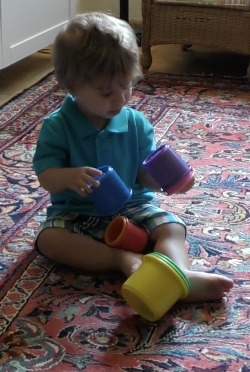
\includegraphics[scale=0.05, height=90mm]{img/grasp.png}
\vspace{0.3em}
\end{center}

}
%%%%%%%%%%%%%%%%%%%%%%%%%%%%%%%%%%%%%%%%%%%%%%%%%%%%%%%%%%%%%%%%%%%%%%%%%%%%%%
\headerbox{Results and Discussion}{name=results, column=1, span=1, below=displays}
%%%%%%%%%%%%%%%%%%%%%%%%%%%%%%%%%%%%%%%%%%%%%%%%%%%%%%%%%%%%%%%%%%%%%%%%%%%%%%
    {
\par 

\par Based on the graph and tables, it can be observed that there is no clear bias between the three age groups regarding amount of times the left, right and both hands were used. This data does not support the idea that duration of interaction and grasp type relates to motor development in infants and toddlers. 
Although these variables do not relate to motor development, several other variables could be studied to further study motor development, such as types of actions the children perform with the toy. 
}
%%%%%%%%%%%%%%%%%%%%%%%%%%%%%%%%%%%%%%%%%%%%%%%%%%%%%%%%%%%%%%%%%%%%%%%%%%%%%%
\headerbox{Figure 1: Grasp durations by type}{name=fig1, column=2, row=0, span=2}
%%%%%%%%%%%%%%%%%%%%%%%%%%%%%%%%%%%%%%%%%%%%%%%%%%%%%%%%%%%%%%%%%%%%%%%%%%%%%%
    {
 \begin{center}
 \vspace{0.3em}
 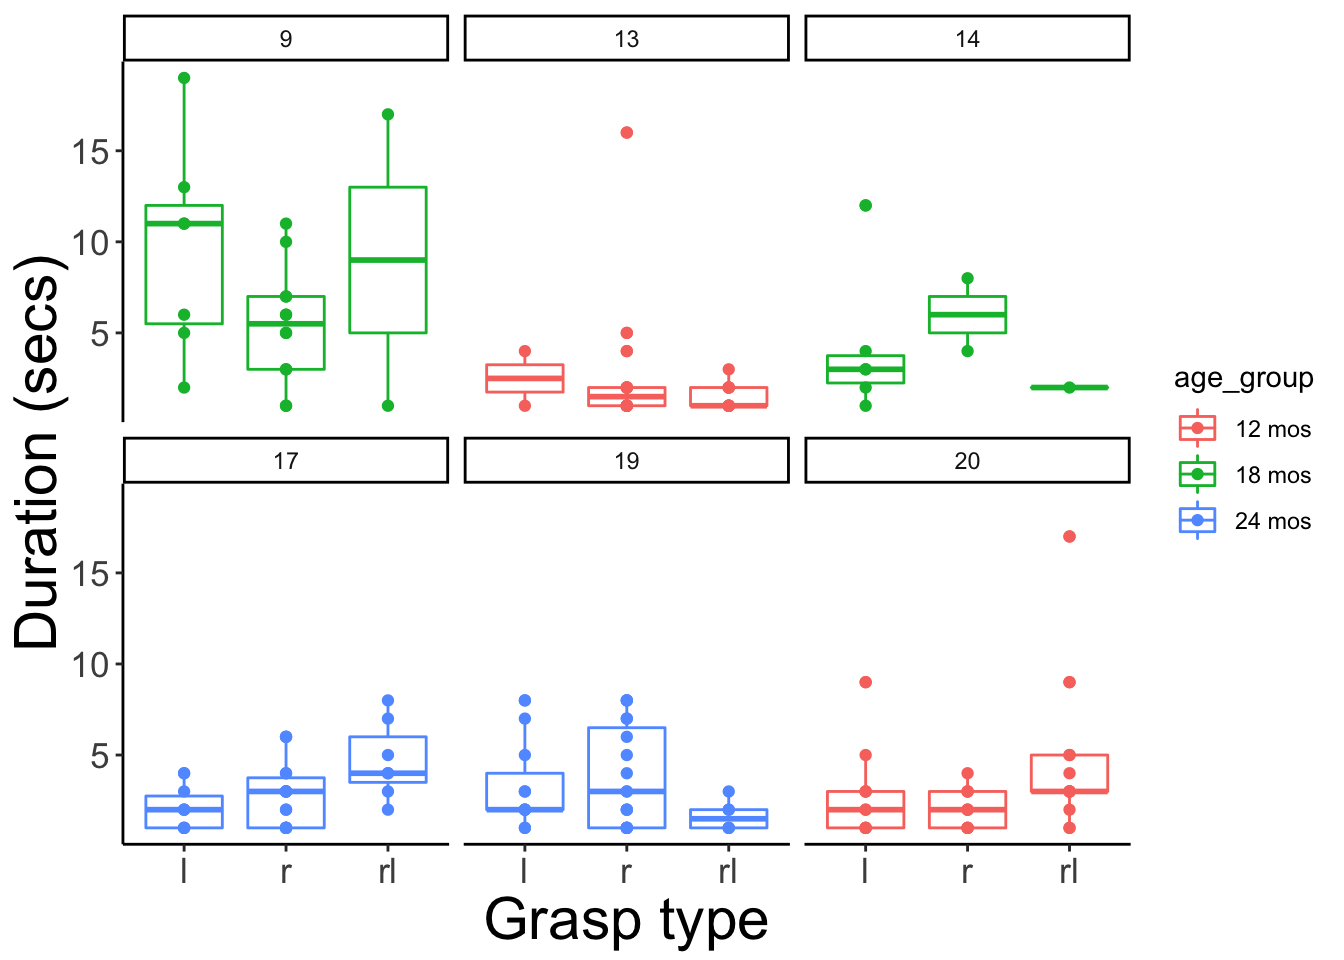
\includegraphics[scale=0.35,valign=t]{hand-touch-which-hand-1.png}
 \vspace{0.3em}
 \end{center}
 }

%%%%%%%%%%%%%%%%%%%%%%%%%%%%%%%%%%%%%%%%%%%%%%%%%%%%%%%%%%%%%%%%%%%%%%%%%%%%%%
\headerbox{Table 1: Grasp counts by type}{name=tab1, column=2, span=2, below=fig1}
%%%%%%%%%%%%%%%%%%%%%%%%%%%%%%%%%%%%%%%%%%%%%%%%%%%%%%%%%%%%%%%%%%%%%%%%%%%%%%
{
\begin{center}
\vspace{0.3em}
\begin{tabular}{ | m{5em} | m{1cm}| m{1cm} | m{1cm} | m{1cm} | m{1cm} | m{1cm} |} 
\hline
grasp type &9 & 13 & 14 & 17 & 19 & 20 \\ 
\hline
l & 7 & 2 & 6 & 10 & 11 & 11\\ 
\hline
r & 12 & 16 & 2 & 18 & 19 & 11 \\ 
\hline
lr & 2 & 11 & 1 & 7 & 6 & 13 \\
\hline
\end{tabular}
\vspace{0.3em}
\end{center}
}

%%%%%%%%%%%%%%%%%%%%%%%%%%%%%%%%%%%%%%%%%%%%%%%%%%%%%%%%%%%%%%%%%%%%%%%%%%%%%%
  \headerbox{Acknowledgements}{name=thanks, column=1, below=results, above=bottom}
%%%%%%%%%%%%%%%%%%%%%%%%%%%%%%%%%%%%%%%%%%%%%%%%%%%%%%%%%%%%%%%%%%%%%%%%%%%%%%
    {
   \small
      This material is based upon work supported by the the National Institutes of Health under Grant Number 1U01HD076595-01.
      Any opinions, findings, and conclusions or recommendations expressed in this material are those of the author(s) and do not necessarily reflect the views of the National Institutes of Health.
    }

%%%%%%%%%%%%%%%%%%%%%%%%%%%%%%%%%%%%%%%%%%%%%%%%%%%%%%%%%%%%%%%%%%%%%%%%%%%%%%
   \headerbox{Data Sharing}{name=sharing, column=2, below=tab1, above=bottom}
%%%%%%%%%%%%%%%%%%%%%%%%%%%%%%%%%%%%%%%%%%%%%%%%%%%%%%%%%%%%%%%%%%%%%%%%%%%%%%%
    {
    \smaller
    
       Movies of the displays, metadata about the participants, and raw data files are available at: \url{https://nyu.databrary.org/volume/444}. This is a private repository. Full reports of our data analysis workflows are available at: \url{http://github.com/gilmore-lab/psi-chi-2019}
       }

%%%%%%%%%%%%%%%%%%%%%%%%%%%%%%%%%%%%%%%%%%%%%%%%%%%%%%%%%%%%%%%%%%%%%%%%%%%%%%
 \headerbox{References}{name=refs, column=3, span=1, below=tab1, above=bottom}
%%%%%%%%%%%%%%%%%%%%%%%%%%%%%%%%%%%%%%%%%%%%%%%%%%%%%%%%%%%%%%%%%%%%%%%%%%%%%%
  {
  %For use with external .bib file
  
  \tiny
  
          \renewcommand{\refname}{\vspace{-0.5em}} % removes "References" canned text.
          \bibliographystyle{IEEEtran}
          \bibliography{IEEEabrv,poster_landscape}
          
}
\end{poster}
\end{document}
